\documentclass[12pt, titlepage]{article}

\usepackage{booktabs}
\usepackage{xr-hyper}
\usepackage{tabularx}
\usepackage{graphicx}
\graphicspath{{../../src/TestCase/}}
\usepackage{hyperref}
\hypersetup{
    colorlinks,
    citecolor=black,
    filecolor=black,
    linkcolor=red,
    urlcolor=blue
}

%% Comments

\usepackage{color}

\newif\ifcomments\commentstrue

\ifcomments
\newcommand{\authornote}[3]{\textcolor{#1}{[#3 ---#2]}}
\newcommand{\todo}[1]{\textcolor{red}{[TODO: #1]}}
\else
\newcommand{\authornote}[3]{}
\newcommand{\todo}[1]{}
\fi

\newcommand{\wss}[1]{\authornote{blue}{SS}{#1}}
\newcommand{\an}[1]{\authornote{magenta}{Author}{#1}}

\externaldocument{../TestPlan/TestPlan}
\externaldocument{../SRS/SRS}
\newcommand{\progname}{SpectrumImageAnalysisPy}

\newcounter{reqnum} %Requirement Number
\newcommand{\rthereqnum}{P\thereqnum}
\newcommand{\rref}[1]{R\ref{#1}}

\begin{document}

\title{Test Report: Project Title} 
\author{Isobel Bicket}
\date{\today}
	
\maketitle

\pagenumbering{roman}

\section{Revision History}

\begin{tabularx}{\textwidth}{p{4cm}p{2cm}X}
\toprule {\bf Date} & {\bf Version} & {\bf Notes}\\
\midrule
December 18, 2017 & 1.0 & Initial draft\\
\bottomrule
\end{tabularx}

~\newpage

\section{Symbols, Abbreviations and Acronyms}
See \hyperref[Doc:SRS]{SRS} document for further definitions.\\

\renewcommand{\arraystretch}{1.2}
\begin{tabular}{l l} 
  \toprule		
  \textbf{symbol} & \textbf{description}\\
  \midrule 
  RMS & Root Mean Square\\
  SNR & Signal-to-Noise Ratio\\
  T & Test\\
  \bottomrule
\end{tabular}\\


\newpage

\tableofcontents

\listoftables %if appropriate

\listoffigures %if appropriate

\newpage

\pagenumbering{arabic}

This document details the results of the testing detailed in the
\hyperref[Doc:TestPlan]{Test Plan}, for the code \progname, which can be found,
along with the other documentation, on
\url{https://github.com/icbicket/SpectrumImageAnalysisPy/tree/SpectrumImageAnalysisPy_dev}. 
Data and results from testing can be found under 
\url{/home/isobel/Documents/McMaster/PythonCodes/DataAnalysis/src/TestCase}.

\section{Functional Requirements Evaluation}
\subsection{\rref{R_SI_inputs}: SI Inputs}

\subsection{\rref{R_spectrum_inputs}: Spectrum Inputs}

\subsection{\rref{R_Input_dimension}: Input Verification}

\subsection{\rref{R_SI_slicing}: Slice (1D) SI and extract Image}

\subsection{\rref{R_SI_area}: Mask (2D) SI and extract Spectrum}

\subsection{\rref{R_deconvolution}: Richardson-Lucy Deconvolution}
The test data for testing the RMS error and SNR of the deconvolution algorithm were obtained from Dr. E.P.Bellido and are the same datasets used in \cite{bellido_toward_2014}.
\begin{figure}
    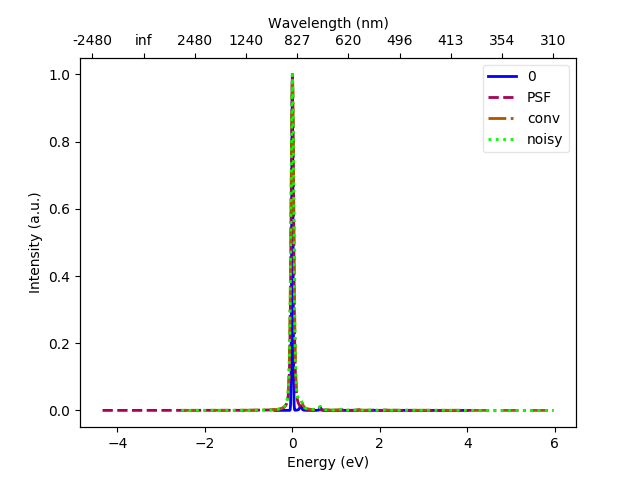
\includegraphics[scale=0.4]{Reference_spectra.png}
    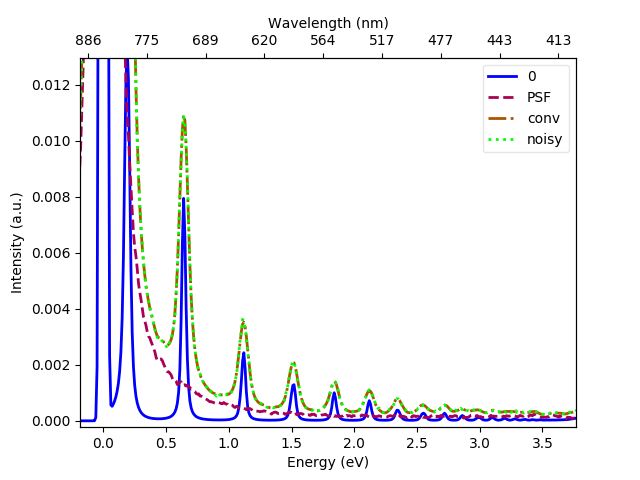
\includegraphics[scale=0.4]{Reference_spectra2.png}
    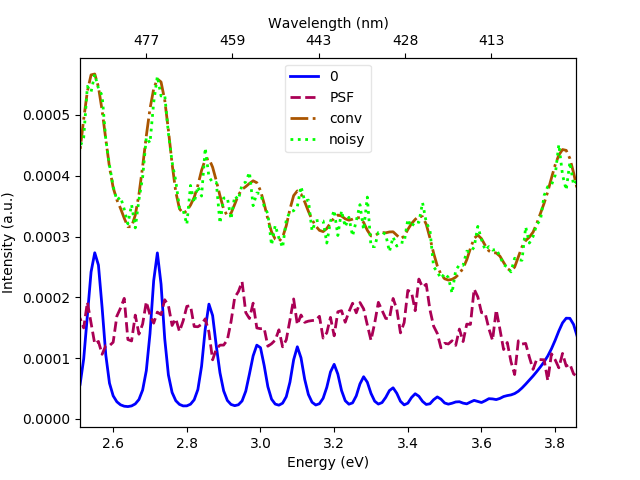
\includegraphics[scale=0.4]{Reference_spectra3.png}
    \caption{Original spectrum (0), Point spread function (PSF), the original spectrum convolved with the PSF (conv), and the original spectrum convolved with the PSF with Poisson noise added (noisy). Three images show three different regions of the spectrum.}
\end{figure}
\begin{figure}[h]
    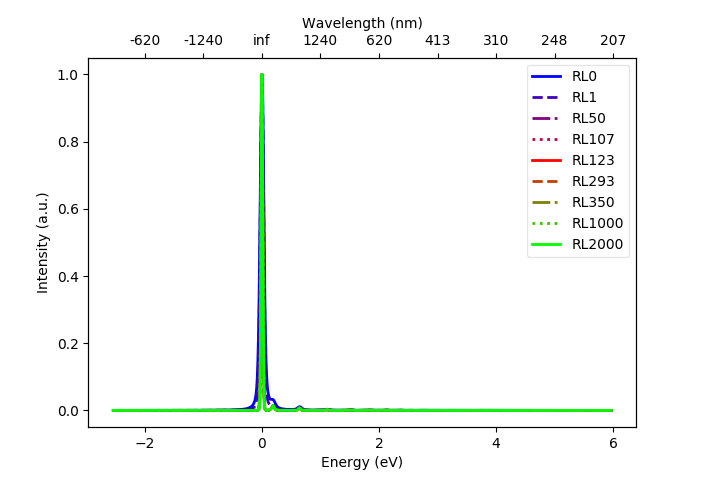
\includegraphics[scale=0.4]{Deconvolved_spectra_SimNoise3.png}
    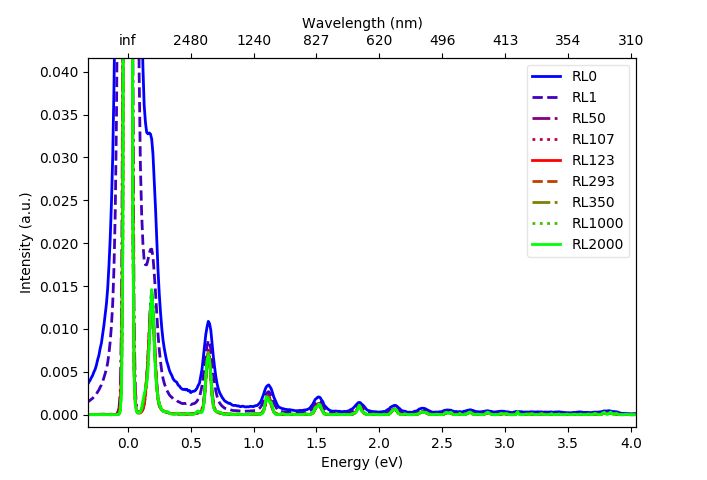
\includegraphics[scale=0.4]{Deconvolved_spectra_SimNoise3-2.png}
    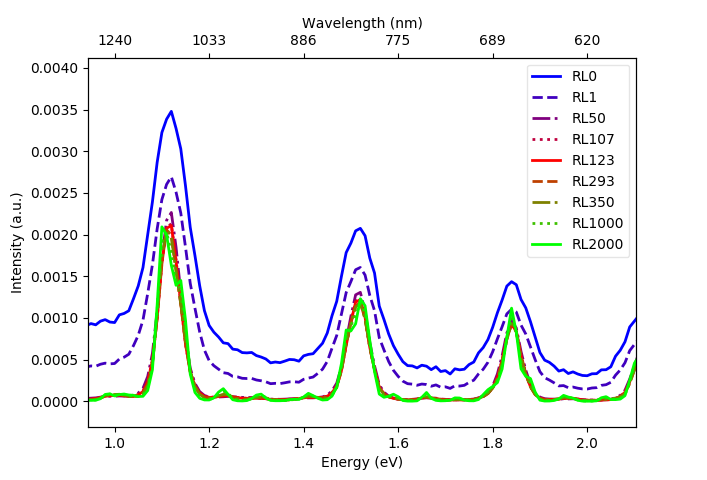
\includegraphics[scale=0.4]{Deconvolved_spectra_SimNoise3-3.png}
    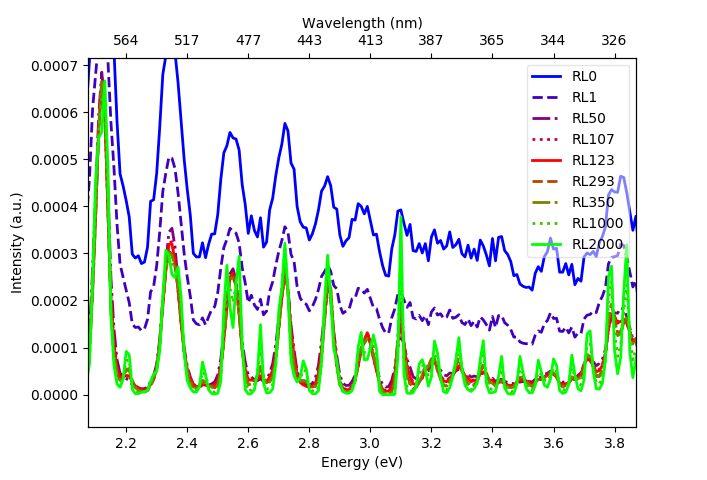
\includegraphics[scale=0.4]{Deconvolved_spectra_SimNoise3-4.png}
    \caption{Spectra deconvolved using the Richardson-Lucy algorithm. Different numbers of iterations were used, as shown in the legend (RL2000 = 2000 iterations). Four images show different regions of the same plot.}
\end{figure}


\subsection{\rref{R_normalization}: Normalization}

\subsection{\rref{R_background}: Background subtraction}

\subsection{\rref{R_gain}: Gain Correction}

\section{Nonfunctional Requirements Evaluation}

\subsection{Usability}
		
\subsection{Performance}

\subsection{etc.}
	
\section{Comparison to Existing Implementation}	

This section will not be appropriate for every project.

\section{Unit Testing}
To date, partial unit testing has been performed on the following files:
\begin{itemize}
    \item Filenamer.py, used to name the files to be exported and avoid conflicts with already existing files).
    \item Spectrum.py, used to implement the Data 1D Spectrum module.
    \item SpectrumImage.py, used to implement the Data 3D Spectrum module
    \item ImagePlotter.py, implementing the Display 2D Image module.
\end{itemize}

Coverage statistics for these files can be found in \hyperref[ssec:StatCov]{Statement Coverage} and \hyperref[ssec:BrCov]{Branch Coverage}.

\section{Changes Due to Testing}
\begin{itemize}
    \item A zero in the denominator during RL deconvolution now raises an exception
\end{itemize}
\section{Automated Testing}
		
\section{Trace to Requirements}
		
\section{Trace to Modules}		

\section{Code Coverage Metrics}
Code coverage metrics were obtained using the Python coverage library (coverage.py-4.4.2) and represent the statement and branch coverage of the unit tests, to date.

\subsection{Statement Coverage}
Statement coverage provides a value for the percentage of lines which were run during the unit tests.

\label{ssec:StatCov}
\begin{table}[h!]
    \centering
    \begin{tabular}{|c|c|c|c|}
        \hline
        Name & Statements & Missed & Coverage \%\\
        \hline
        FileNamer.py & 40 & 3 & 92\%\\
        ImagePlotter.py & 136 & 97 & 29\%\\
        SpectrumImage.py & 247 & 155 & 37\%\\
        Spectrum.py & 136 & 70 & 49\%\\
        \hline
    \end{tabular}
    \caption{Statement coverage}
    \label{Table:Statementcov}
\end{table}

\subsection{Branch Coverage}
\label{ssec:BrCov}
Branch coverage combines the number of statements run during the test with the number of branches covered during the test.
\begin{table}[h!]
    \centering
    \begin{tabular}{|c|c|c|c|c|c|}
        \hline
        Branch Name & Statements & Missed & Branches & Partial Branches & Coverage \%\\
        \hline
        FileNamer.py & 40 & 3 & 14 & 1 & 93\%\\
        ImagePlotter.py & 136 & 97 & 56 & 0 & 23\%\\
        SpectrumImage.py & 247 & 155 & 60 & 1 & 37\%\\
        Spectrum.py & 136 & 70 & 32 & 1 & 48\%\\
        \hline
    \end{tabular}
    \caption{Branch coverage}
    \label{Table:Branchcov}
\end{table}

\newpage
\bibliographystyle{ieeetr}

\bibliography{TestReport}

\end{document}